\subsection{Impact of Misjudging the Completeness of the Data Set} \label{sec:results_incompR}

The selection function (see Section \ref{sec:selectionfunction}) can be very complex and is therefore sometimes not perfectly known. Here we investigate how much this could affect the recovery of the potential. We do this by creating mock data in a spherical survey volume around the Sun with a spatially varying incompleteness function, while assuming constant completeness in the \RM{} analysis. Our test case uses a completeness function which drops linearly with distance $r$ from the Sun (see Test \ref{test:isoSphFlexIncomp} in Table \ref{tbl:tests} and Figure \ref{fig:isoSphFlexIncomp_completeness_shapes}). This captures the relevant case of stars being less likely to be observed (than assumed) the further away they are (e.g. due to unknown dust obscuration). 

Figure \ref{fig:isoSphFlexIncompR_violins} demonstrates that the potential recovery with \RM{} is very robust against somewhat wrong assumptions about the radial completeness of the data. The robustness for the \texttt{cool} stellar population is even more striking than for the \texttt{hot} population. The reason for this robustness could be, that much information about the potential comes from the rotation curve measurements in the plane, which is not affected by the incompleteness of the sample. We test this by not including tangential velocity measurements in the analysis of the data sets from Figure \ref{fig:isoSphFlexIncompR_violins} (by marginalizing the likelihood in Equation \ref{eq:prob} over $v_T$). Figure \ref{fig:isoSphFlexIncompR_marginal_violins} shows that in this case the potential is much less tightly constrained, even for 20,000 stars. For only small deviations of true and assumed completeness ($\lesssim 10\%$) we can however still incorporate the true potential in our fitting result (see Figure \ref{fig:isoSphFlexIncomp_marginal_violins}).

We found similar results also for spatial incompleteness functions varying with $z$

\HW{[TO DO: Comment by HW: I don't have an immediate solution for this, but again, it seems the interesting question of "how much of the information is in the rotation curve" is 'hidden' in the section on selection functions... - What does he mean by that?]}


%=============================




\begin{figure}[!htbp]
\centering
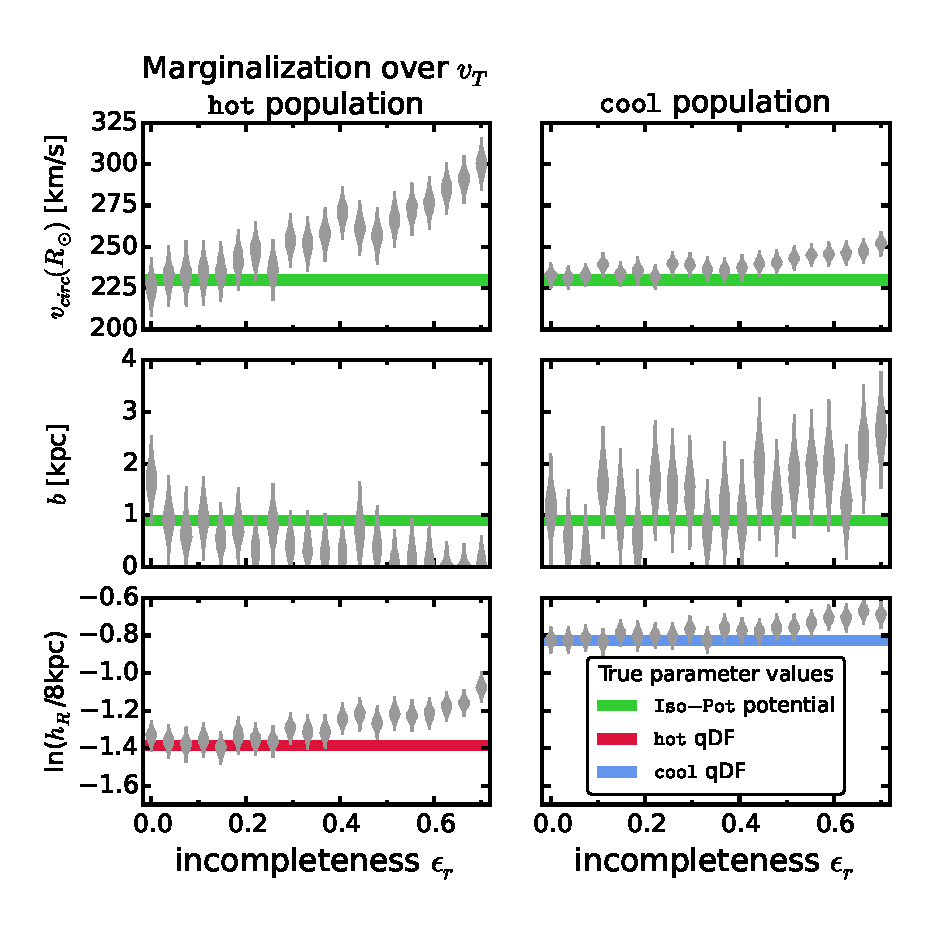
\includegraphics[width=\columnwidth]{figs/isoSphFlexIncompR_marginal_violins_3.eps}
\caption{Same as Figure \ref{fig:isoSphFlexIncompR_violins}, but without including information about the tangential velocities in the analysis. This was done by marginalizing the likelihood in Equation \ref{eq:prob} over $v_T$. The parameter recovery is much worse than in Figure \ref{fig:isoSphFlexIncompR_violins} (as can be seen from comparing the parameter ranges on the $y$-axis). This could indicate that much of the information about the potential is actually stored in the rotation curve, i.e. $v_T(R)$, which is not affected by removing stars from the data set. But even if we do not include $v_T$ we can still recover the potential within the errors, at least for small ($\epsilon_z \lesssim 10\%$).} 
\label{fig:isoSphFlexIncompR_marginal_violins}
\end{figure}

\Wilma{[TO DO: Remove vertical incompleteness from test table]}
